\chapter{Introduction}\label{chap:intro}

\section{Background History}
Hello and welcome, \ac{UniMAP} FYP students!  The \verb|unimapcgsfyp| class and template files were written in the hope that they may help you prepare your research thesis using \LaTeX, based on the \ac{CGS} requirements \citep{cgs:thesis:guideline:2017}. \textbf{Please note that this version is based on the guidelines, in force 2017 onwards.} Also, I would like to give credit to Lim Lian Tze, where this document class is created based on her \emph{usmthesis.cls} \cite{lim:2007}. The explanation beyond this paragraph also heavily edited based on her \emph{usmthesis.cls} document class. 

If you prefer the acronym to be written in full like it was mentioned first time, use \verb|\acf{youracronym}|. Subsequently, you use the usual \verb|\ac{youracronym}|. Remember the acronym for \acf{UniMAP}?. 

\LaTeX{} is powerful and produces beautiful documents.  However, there is definitely a learning curve to it -- one that is worth the effort.  %This is also a learning process for the author, so 
If you find any errors in these templates or documents \citep{matsom:template}, or have any suggestions or feedback, do e-mail me about it (\path{msmhanafi@gmail.com}).  The author cannot always guarantee prompt response, however. %\Smiley

MiK\TeX{}, my recommended \LaTeX{} distribution for Windows, is available on the \url{https://miktex.org/howto/install-miktex}. Macbook users can opt to install MacTeX \url{http://www.tug.org/mactex/}. The complete version of MacTeX (over 2 gigabytes of material) installs TeXShop, a GUI front end to TeX, TeX Live 2019, a GUI front end to manage \LaTeX~core and packages, and other important materials. The basic version of MacTeX is lightweight (around 110 megabytes) but require user to install TeX Live 2019 separately.

\section{Samples of Basic \LaTeX{}}

There are plenty of free \LaTeX{} tutorials online.  This sample thesis includes some examples to do some common tasks.  We start with some examples for lists (both bulleted and numbered), highlighting texts in bold and italic, and URLs:

\lstset{breaklines=true, basicstyle=\small\ttfamily, language=[LaTeX]TeX, columns=fullflexible, framesep=10pt, xleftmargin=16pt, keywordstyle={\mdseries}}

\begin{figure}[htb!]
\begin{lstlisting}
\begin{enumerate}
\item bulleted and numbered lists, 
\item font effects such as

\begin{itemize}
\item \textbf{bold}, 
\item \emph{italic}, and 
\item \texttt{typewriter-like}
\end{itemize}

\item URLs and e-mail addresses: \url{http://www.mohdhanafi.unimap.edu.my/template}, \url{dummy.add@outlook.com};
\item citations: see Chapter \ref{chap:review}.
\end{enumerate}
\end{lstlisting}
\caption{Common Layout and Formatting Tasks. Note how this long title wraps around I hope it works anyway. Look it needs more, so here's some more longer text. Is that enough? I hope it is.}\label{fig:simple}
\end{figure}

\begin{enumerate}
\item bulleted and numbered lists, 
\item font effects such as

\begin{itemize}
\item \textbf{bold}, 
\item \emph{italic}, and 
\item \texttt{typewriter-like}
\end{itemize}

\item URLs and e-mail addresses:\\ \url{http://www.mohdhanafi.unimap.edu.my/template}, \url{dummy@outlook.com};
\item citations: see Chapter \ref{chap:review}
\end{enumerate}

Incidentally, if you feel that the lists above are too far apart vertically, you can customize them using the \texttt{enumitem} package. The effect is then like the following:

\begin{figure}[htb!]
\begin{lstlisting}
\begin{enumerate}[nosep]
\item item one,
\item item two,
\item item three.
\end{enumerate}

\begin{itemize}[nosep]
\item item one,
\item item two,
\item item three.
\end{itemize}
\end{lstlisting}
\caption{Compact Lists}\label{fig:enumitem}
\end{figure}


\begin{enumerate}[nosep]
\item item one,
\item item two,
\item item three.
\end{enumerate}

\begin{itemize}[nosep]
\item item one,
\item item two,
\item item three.
\end{itemize}

Granted, the lists are still wide, but this is because we need to honour the requirement for double line-spacing. If allowable, then you can do the list in single line-spacing.

\begin{figure}[htb!]
	\begin{lstlisting}
	\begin{enumerate}[nosep]\singlespacing
		\item item one,
		\item item two,
		\item item three.
	\end{enumerate}
	
	\begin{itemize}[nosep]\singlespacing
		\item item one,
		\item item two,
		\item item three.
	\end{itemize}
	\end{lstlisting}
	\caption{Compact Lists and single spacing}\label{fig:enumitemsinglespacing}
\end{figure}


\begin{enumerate}[nosep]\singlespacing
	\item item one,
	\item item two,
	\item item three.
\end{enumerate}

\begin{itemize}[nosep]\singlespacing
	\item item one,
	\item item two,
	\item item three.
\end{itemize}

If, for some reasons, you want to change the look of your numbered list or bullet shape, you can refer to this post \href{https://texblog.org/2008/10/16/lists-enumerate-itemize-description-and-how-to-change-them/}{\texttt{https://texblog.org/lists-enumerate-itemize/}} and \url{http://www.texnia.com/archive/enumitem.pdf}. For examples, you can change to number with parenthesis \verb|(\arabic*)|, alphabet \verb|\alph*| or \verb|Alph*|, roman style \verb|\roman*| or \verb|\Roman*|             

\begin{figure}[htb!]
	\begin{lstlisting}
	\begin{enumerate}[nosep,label=(\arabic*)]\singlespacing
		\item item one,
		\item item two.
	\end{enumerate}
	
	\begin{enumerate}[nosep,label=(\alph*)]\singlespacing
		\item item one,
		\item item two.
	\end{enumerate}
	
	\begin{enumerate}[nosep,label=\Roman*)]\singlespacing
		\item item one,
		\item item two.
	\end{enumerate}
	\end{lstlisting}
	\caption{Compact Lists, single spacing, and change the numbered format}\label{fig:enumitemchangeformatsinglespacing}
\end{figure}

\begin{enumerate}[nosep,label=(\arabic*)]\singlespacing
	\item item one,
	\item item two.
\end{enumerate}

\begin{enumerate}[nosep,label=(\alph*)]\singlespacing
	\item item one,
	\item item two.
\end{enumerate}

\begin{enumerate}[nosep,label=\Roman*)]\singlespacing
	\item item one,
	\item item two.
\end{enumerate}


\section{Dimensions in \LaTeX{}}
Examples of dimension in \LaTeX{} are given in Figure~\ref{fig:dimentionLatex}.

\begin{figure}[hbt!]\centering
	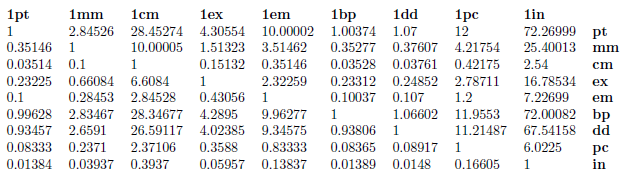
\includegraphics[scale=0.75]{dimentionLatex}
	\caption{Dimension in \LaTeX{}} \label{fig:dimentionLatex}
\end{figure}

\section{Special Characters}

Bear in mind that certain characters are special \LaTeX{} symbols and need to be escaped, as shown in Table~\ref{tab:special:char}.

\begin{table}[htb!]
\caption{Special Characters in \LaTeX}\label{tab:special:char}
\centering
\begin{singlespace}\begin{tabular}{|c | l | l|}
\hline
Symbol & Name & Escape code \\\hline\hline
\# & \normalsize{hash, pound} & \verb|\#| \\
\$ & \normalsize{dollar} & \verb|\$| \\
\% & \normalsize{percent} & \verb|\%| \\
\^{} & \normalsize{``hat''} & \verb|\^{}| \\
\& & \normalsize{ampersand} & \verb|\&| \\
\_ & \normalsize{underscore} & \verb|\_| \\
\{ & \normalsize{left brace} & \verb|\{| \\
\} & \normalsize{right brace} & \verb|\}| \\
\~{} & \normalsize{tilde} & \verb|\~{}| \\
$\sim$ & \normalsize{wide tilde} & \verb|$\sim$| \\
`` & \normalsize{open double quotes} & \verb|``| \\
'' & \normalsize{close double quotes} & \verb|''| \\
\hline
\end{tabular}\end{singlespace}
\end{table}

Note that for quotation marks, you might prefer \verb|``this'' and `that'|  (``this'' and `that')
instead of \verb|"this" and 'that'|  ("this" and 'that'). The symbol \verb|`| can be found below \verb|esc| keyboard, together with tilde \verb|~| symbol. 

If you need to typeset special characters (such as $\curvearrowright$, etc), take a look at the left side on the navigation panel of the TeXstudio. If you installed MiKTeX on a Windows machine, Comprehensive \LaTeX\ Symbol List  could be found under \path|C:\Program Files\MiKTeX 2.9\doc\info\symbols\comprehensive\symbols-a4.pdf|. 


\section{Useful Resources}\label{sec:resources}
\citet{latex:companion} is a \emph{very} useful book --- but it's quite an investment at RM180++.  A worthy one, nevertheless.  \citet{roberts} has a website with very good \LaTeX{} tutorials at \url{http://www.comp.leeds.ac.uk/andyr/misc/latex/}, too.  Don't forget the famous \texttt{lshort} \url{https://tobi.oetiker.ch/lshort/lshort.pdf} tutorial \citep{lshort}. 

You can also find the list compiled by Lim Lian Tze (the template owner of \verb|usmthesis.cls|, which this thesis is based on) at \href{http://liantze.penguinattack.org/latextypesetting}{\texttt{http://liantze.penguinattack.org/latextypesetting}} \citep{lim:latextypesetting}. Also, on my website \href{http://mohdhanafi.unimap.edu.my/template}{\texttt{http://mohdhanafi.unimap.edu.my/}}\citep{matsom:template}.

\section{Useful Tips} %https://www.mackichan.com/index.html?techtalk/395.htm~mainFrame
You might encounter where the section heading in the table of contents appear at the bottom of the page. You can force a page break before a table of content entry. Place an insertion point above the heading in the document, then type \verb|\addtocontents{toc}{\protect\pagebreak}|. Recompile the document and you can see the change on the table of contents.

\noindent For example, the Chapter 3 header appear at the bottom of the page. 

\begin{lstlisting}
	\addtocontents{toc}{\protect\pagebreak}
	\chapter{Figures, Tables, Equations, Algorithms, etc}\label{chap:design}
\end{lstlisting}

If you encounter problems, please make use of google. Start by searching \verb|latex yourproblem|. For example, \verb|latex figure size|. 
	